\documentclass[aspectratio=1610,handout=false, tikz,border=10pt]{beamer}
\usepackage{circuitikz}
\usepackage{kantlipsum}
\usepackage{smartdiagram}
\usepackage{pgfplots}
\usepackage{etex}
\usetikzlibrary{pgfplots.groupplots}
\pgfplotsset{compat=1.18}
\usetikzlibrary{arrows.meta, calc, positioning, shapes.geometric, arrows}


\usetheme[progressbar=frametitle]{metropolis}
\usepackage{appendixnumberbeamer}
\usepackage{xcolor}
\tikzstyle{box} = [rectangle, draw, text centered, minimum height=1cm, minimum width=3cm]
\tikzstyle{startstop} = [rectangle, rounded corners, minimum width=3.5cm, minimum height=1cm, text centered, draw=black, fill=white, font=\footnotesize]
\tikzstyle{process} = [rectangle, rounded corners, minimum width=2.5cm, minimum height=1cm, text centered, draw=black, fill=white]
\tikzstyle{database} = [cylinder, shape border rotate=90, draw, fill=red!20, text centered, minimum height=1.5cm, minimum width=0.8cm, aspect=0.25]
\tikzstyle{arrow} = [thick,->,>=stealth]
\tikzstyle{arrow_bend} = [thick,->,>=stealth, bend left]


\usepackage{graphicx} % Required for including images

% Set the path for the images folder
\graphicspath{{images/}}




\usepackage{tikz}
\usetikzlibrary{shapes.geometric, arrows, positioning, fit, backgrounds, calc, arrows.meta}
\tikzstyle{startstop} = [rectangle, rounded corners, minimum width=3cm, minimum height=1cm,text centered, draw=black, fill=red!30]
\tikzstyle{process} = [rectangle, minimum width=3cm, minimum height=1cm, text centered, draw=black, fill=blue!30]
\tikzstyle{decision} = [diamond, minimum width=3cm, minimum height=1cm, text centered, draw=black, fill=green!30]
\tikzstyle{arrow} = [thick,->,>=stealth]
\usepackage{xcolor}




\usepackage[utf8]{inputenc}

\usepackage{booktabs}
\usepackage[scale=2]{ccicons}

\usepackage{pgfplots}
\usepgfplotslibrary{dateplot}

\usepackage{xspace}
\newcommand{\themename}{\textbf{\textsc{metropolis}}\xspace}
\definecolor{mSybilaRed}{HTML}{990000}

\setbeamercolor{title separator}{
  fg=mSybilaRed
}

\setbeamercolor{progress bar}{%
  fg=mSybilaRed,
  bg=mSybilaRed!90!black!30
}

\setbeamercolor{progress bar in section page}{
  use=progress bar,
  parent=progress bar
}

\setbeamercolor{alerted text}{%
  fg=mSybilaRed
}

\title{Docker Container and Containerization }
\subtitle{Latex presentation CSE-200}
\institute{Bangladesh University of Engineering and Technology}
\date{\today}

\addtobeamertemplate{footline}{}{%
    \begin{picture}(0,0)
        \put(325,25){\includegraphics[width=1cm]{Images/platform-docker-logo.png}} % Adjust position and size
    \end{picture}
    \vspace{0.2cm} % Adjust to align navigation bar
}

\setbeamertemplate{footline}
{
  \leavevmode
  \hbox{
  \begin{beamercolorbox}[wd=.15\paperwidth,ht=2.25ex,dp=1ex,center]{title in head/foot}
    \usebeamerfont{author in head/foot}\insertshortauthor
  \end{beamercolorbox}

  \begin{beamercolorbox}[wd=.7\paperwidth,ht=2.25ex,dp=1ex,center]{author in head/foot}
    \usebeamerfont{author in head/foot}\insertshorttitle
  \end{beamercolorbox}

  \begin{beamercolorbox}[wd=.15\paperwidth,ht=2.25ex,dp=1ex,center]{title in head/foot}
    \insertframenumber{} / \inserttotalframenumber
  \end{beamercolorbox}
  }
}
\definecolor{cloudblue}{rgb}{0.0, 0.5, 1.0}
\definecolor{servergreen}{rgb}{0.0, 0.7, 0.0}
\definecolor{clientred}{rgb}{0.8, 0.2, 0.2}
\definecolor{storageyellow}{rgb}{1.0, 0.8, 0.2}
\definecolor{computeorange}{rgb}{1.0, 0.4, 0.0}
\definecolor{backupgray}{rgb}{0.6, 0.6, 0.6}

\tikzstyle{cloud}=[cloud, draw, fill=cloudblue, cloud puffs=10, cloud puff arc=80, minimum width=7cm, minimum height=5cm]
\tikzstyle{server}=[rectangle, draw, fill=servergreen, minimum width=3cm, minimum height=1.2cm]
\tikzstyle{client}=[circle, draw, fill=clientred, minimum size=1cm]
\tikzstyle{service}=[rectangle, draw, fill=gray!20, minimum width=2.8cm, minimum height=1cm, text centered]
\tikzstyle{connection}=[draw, thick, opacity=0.5, dashed]
\tikzstyle{dataconnection}=[draw, thick, opacity=0.7, red, -latex]
\tikzstyle{firewall}=[rectangle, draw, fill=blue!30, minimum width=4cm, minimum height=1cm, text centered]

\tikzstyle{cblue}=[circle, draw, thin, fill=darkcyan, scale=0.8]
\tikzstyle{qgre}=[rectangle, draw, thin, fill=darkgreen, scale=0.8]
\tikzstyle{rpath}=[ultra thick, darkred, opacity=0.6]

% TikZ styles
\tikzset{
  comp/.style = {
    minimum width  = 2.5cm,
    minimum height = 1.5cm,
    text width     = 4cm,
    inner sep      = 0pt,
    text           = green,
    align          = center,
    font           = \Large,
    transform shape,
    thick
  },
  monitor/.style = {draw = none, xscale = 18/16, yscale = 11/9},
  display/.style = {shading = axis, left color = black!60, right color = black},
  ut/.style      = {fill = gray}
}
\tikzset{
  computer/.pic = {
    % Computer drawing code (unchanged)
    \node(-m) [comp, pic actions, monitor]
      {\phantom{\parbox{\linewidth}{\tikzpictext}}};
    \node[comp, pic actions, display] {\tikzpictext};
    \begin{scope}[x = (-m.east), y = (-m.north)]
      \path[pic actions, draw = none]
        ([yshift=2\pgflinewidth]-0.1,-1) -- (-0.1,-1.3) -- (-1,-1.3) --
        (-1,-2.4) -- (1,-2.4) -- (1,-1.3) -- (0.1,-1.3) --
        ([yshift=2\pgflinewidth]0.1,-1);
      \path[ut]
        (-1,-2.4) rectangle (1,-1.3)
        (-0.9,-1.4) -- (-0.7,-2.3) -- (0.7,-2.3) -- (0.9,-1.4) -- cycle;
      \path[pic actions, fill = none]
        (-1,1) -- (-1,-1) -- (-0.1,-1) -- (-0.1,-1.3) -- (-1,-1.3) --
        (-1,-2.4) coordinate(sw)coordinate[pos=0.5] (-b west) --
        (1,-2.4) -- (1,-1.3) coordinate[pos=0.5] (-b east) --
        (0.1,-1.3) -- (0.1,-1) -- (1,-1) -- (1,1) -- cycle;
      \node(-c) [fit = (sw)(-m.north east), inner sep = 0pt] {};
    \end{scope}
  }
}

% Define the arrows
\def\arrow{
  (10.75:1.1) -- (6.5:1) arc (6.25:120:1) [rounded corners=0.5] --
  (120:0.9) [rounded corners=1] -- (130:1.1) [rounded corners=0.5] --
  (120:1.3) [sharp corners] -- (120:1.2) arc (120:5.25:1.2)
  [rounded corners=1] -- (10.75:1.1) -- (6.5:1) -- cycle
}

\tikzset{
  ashadow/.style={opacity=.25, shadow xshift=0.07, shadow yshift=-0.07},
}

\def\arrows[#1]{         
  \begin{scope}[scale=#1]
    % Draw first circle with arrows and text
    \draw[color=darkred, 
    drop shadow={ashadow, color=red!60!black}] \arrow;
    \node at (-1.6,0.6) {\textcolor{black}{plan}};  % Text placed after the arrow

    \draw[color=darkgreen, bottom color=green!90!black, top color=green!60, 
    drop shadow={ashadow, color=green!60!black}] [rotate=120] \arrow;
    \node at (0,1.5) {\textcolor{black}{code}};  % Text placed after the arrow

    \draw[color=darkblue, right color=blue, left color=blue!60, 
    drop shadow={ashadow, color=blue!60!black}] [rotate=240] \arrow;
     \node at (1,-1.3) {\textcolor{black}{build}};
  \end{scope}

  % Draw second circle with arrows and text, shifted to the right
  \begin{scope}[scale=#1, xshift=4cm]  % Shifted by 6 cm horizontally
    \draw[color=darkred, 
    drop shadow={ashadow, color=red!60!black}] \arrow;
    \node at (-1.8,1) {\textcolor{black}{release}};  % Text placed after the arrow

    \draw[color=darkgreen, bottom color=green!90!black, top color=green!60, 
    drop shadow={ashadow, color=green!60!black}] [rotate=120] \arrow;
    \node at (1,1.5) {\textcolor{black}{deploy}};  % Text placed after the arrow

    \draw[color=darkblue, right color=blue, left color=blue!60, 
    drop shadow={ashadow, color=blue!60!black}] [rotate=240] \arrow;
    \node at (0.8,-1.5) {\textcolor{black}{operator}};
  \end{scope}
  
  % Arrow connecting the two circles
  \draw[->, thick, color=black] (1.2, 0) -- (2.2, 0); 
  \node at (1.6,-0.3){Test}% Arrow from the first circle to the second
}

\definecolor{cloudblue}{rgb}{0.0, 0.5, 1.0}
\definecolor{servergreen}{rgb}{0.0, 0.7, 0.0}
\definecolor{clientred}{rgb}{0.8, 0.2, 0.2}
\definecolor{storageyellow}{rgb}{1.0, 0.8, 0.2}
\definecolor{computeorange}{rgb}{1.0, 0.4, 0.0}
\definecolor{backupgray}{rgb}{0.6, 0.6, 0.6}

\tikzstyle{cloud}=[cloud, draw, fill=cloudblue, cloud puffs=10, cloud puff arc=80, minimum width=7cm, minimum height=5cm]
\tikzstyle{server}=[rectangle, draw, fill=servergreen, minimum width=3cm, minimum height=1.2cm]
\tikzstyle{client}=[circle, draw, fill=clientred, minimum size=1cm]
\tikzstyle{service}=[rectangle, draw, fill=gray!20, minimum width=2.8cm, minimum height=1cm, text centered]
\tikzstyle{connection}=[draw, thick, opacity=0.5, dashed]
\tikzstyle{dataconnection}=[draw, thick, opacity=0.7, red, -latex]
\tikzstyle{firewall}=[rectangle, draw, fill=blue!30, minimum width=4cm, minimum height=1cm, text centered]


\begin{document}
\maketitle

\begin{frame}{Table of contents}
  \setbeamertemplate{section in toc}[sections numbered]
  \tableofcontents[hideallsubsections]
\end{frame}



\section{Introduction}

% \begin{frame}{\textbf{Contents}}
%     \begin{enumerate}
%         \item What is \textbf{Container} and \textbf{Containerization}
%         \item An Analogy
%         \item Docker Introduuction
%         \item Docker : Basic WorkFlow
%         \item Docker : Advantage
%         \item Docker : Disadvantage
%         \item Docker : Interest8ing
        
%     \end{enumerate}
% \end{frame}

% \begin{frame}[plain] % [plain] removes default header/footer
%     \begin{tikzpicture}[remember picture,overlay]
%         % Add background image scaled to fit the slide width
%         \node[opacity=0.15, anchor=center] at (current page.center) {
%             \includegraphics[width=0.88\paperwidth]{Images/Docker Containers.png}
%         };
%     \end{tikzpicture}

%     % Slide content      
%     \frametitle{What is a Container?}
%     \begin{columns}
%         % Left Column: Text
%         \column{0.6\textwidth}
%         \begin{itemize}
%         \setlength\itemsep{1.2em} % Adjust the gap between items, e.g., 1em
%             \item A \textbf{\textcolor{blue}{lightweight, standalone}} software package.

%             \item Ensures \textbf{\textcolor{red}{Isolated environment}}.

%             \item \textbf{\textcolor{green}{Portability and scalability}} for cloud-native and distributed applications.
%         \end{itemize}
        
%         % Right Column: Image
%         \column{0.4\textwidth}
%         \begin{center}
%             % Optionally add an image or icon here
%         \end{center}
%     \end{columns}
    
% \end{frame}

\begin{frame}[plain] % [plain] removes default header/footer
    \begin{tikzpicture}[remember picture,overlay]
        % Add background image scaled to fit the slide width
        \node[opacity=0.15, anchor=center] at (current page.center) {
            \includegraphics[width=0.88\paperwidth]{Images/Docker Containers.png}
        };
    \end{tikzpicture}

    % Slide content      
    \frametitle{What is a Container?}

    \begin{columns}
        % Left Column: Text
        \column{0.6\textwidth}
        \begin{itemize}
        \setlength\itemsep{2em} % Adjust the gap between items
        
            \onslide<1> 
            \item \textbf{\textcolor{blue}{\Large Lightweight, standalone}} software package.

            \onslide<2>
            \item Ensures \textbf{\textcolor{red}{\Large Isolated environment}}.

            \onslide<3>
            \item \textbf{\textcolor{green}{\Large Portability and scalability}} for cloud-native and distributed applications.
            
        \end{itemize}
        
        % Right Column: Placeholder for an image or icon
        \column{0.4\textwidth}
        \begin{center}
            % Optionally add an image or icon here
        \end{center}
    \end{columns}
    
\end{frame}



\begin{frame}[plain] % [plain] removes default header/footer
    \begin{tikzpicture}[remember picture,overlay]
        % Add background image scaled to fit the slide width
        \node[opacity=0.15, anchor=center] at (current page.center) {
            \includegraphics[width=0.88\paperwidth]{Images/Docker Containers.png}
        };
    \end{tikzpicture}

    % Slide content      
    \frametitle{What is Containerization?}
    \begin{columns}
        % Left Column: Text
        \column{0.6\textwidth}
        \begin{itemize}
        \setlength\itemsep{1.2em} % Adjust the gap between items, e.g., 1em
            \item \textbf{\textcolor{orange}{\Large Packaging applications}} with all dependencies.  

            \item \textbf{\textcolor{red}{\Large Ensures consistent}} execution across environments.  

            \item \textbf{\textcolor{green}{\Large Enables scalability}} and efficient deployment.
        \end{itemize}
        
        % Right Column: Image
        \column{0.4\textwidth}
        \begin{center}
        \end{center}
    \end{columns}
    
\end{frame}


% \begin{frame}
% \frametitle{\textbf{An Analogy}}
% \vspace{-2em} % Move the list upwards
% \begin{itemize}
%     \item {\color{blue} \Large Before 1960, most cargo was shipped break bulk. Shippers and carriers alike needed to worry about bad interactions between different types of cargo (e.g., if a shipment of anvils fell on a sack of bananas).}
%     \vspace{1cm}
%     \item {\color{red} \Large Similarly, transitions between different modes of transport were painful.}
% \end{itemize}
% \end{frame}


\begin{frame}
\frametitle{An Analogy}
\textbf{Before 1960, Cargo Transitions between different modes of transport were painful}
\begin{figure}[h]
    \centering
    \includegraphics[width=0.65\textwidth]{Images/Analogy1.png}
    \caption{Multiplicity of Goods and transportation}
    \label{fig:enter-label}
\end{figure}

\end{frame}


% \begin{frame}{\textbf{An Analogy}}

% \vspace{-2em} % Move the list upwards
% \begin{itemize}
%     \item {\color{blue} \Large The answer was found in form of a \textbf{Standard shipping Container}
%     \vspace{1cm}
%     \item {\color{red} \Large Similarly, transitions between different modes of transport were painful.}
% \end{itemize}
% \end{frame}


\begin{frame}
\frametitle{An Analogy}
\textbf{The answer was found in the form of a shipping container.}
\begin{figure}
    \centering
    \includegraphics[width=0.8\linewidth, height =0.5\linewidth ]{Images/Analogy2.2.png}
    \caption{Multiplicity of Goods and transportation}
    \label{fig:enter-label}
\end{figure}   
\end{frame}


\begin{frame}
\frametitle{An Analogy}
\textbf{ Similarly, Docker is a shipping container for code}
\begin{figure}
    \centering
    \includegraphics[width=0.7\linewidth, height =0.5\linewidth ]{Images/Analogy3.2.png}
    \caption{Docker Container}
    \label{fig:enter-label}
\end{figure}
    
\end{frame}
\begin{frame}[plain]
    \frametitle{\textbf{Virtualization vs Containerization}}
    
    \begin{center}
    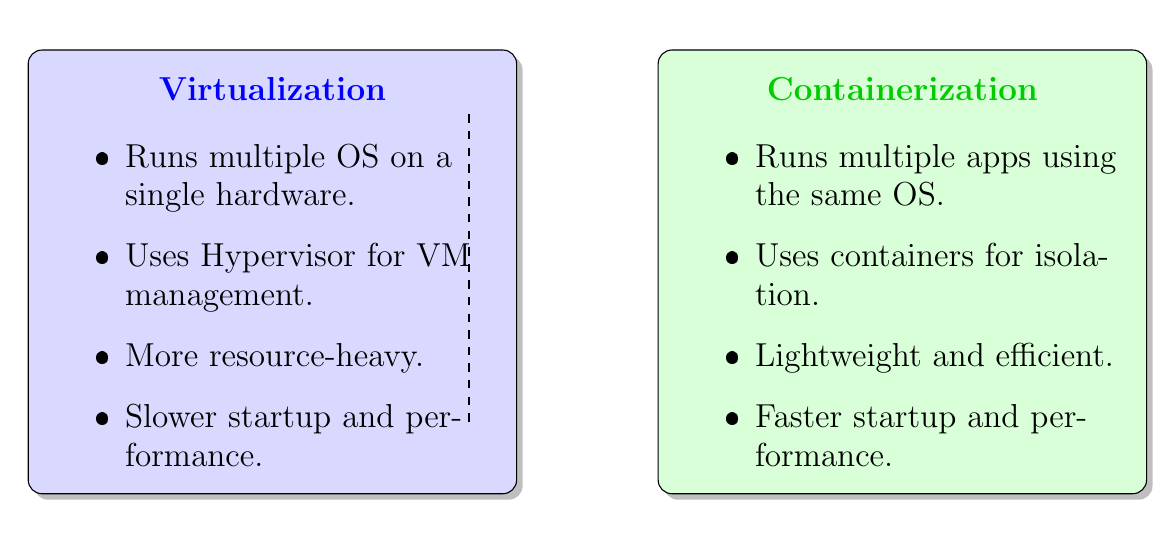
\begin{tikzpicture}[
        every node/.style={minimum width=6cm, minimum height=4cm, align=center, text width=5.5cm, font=\large, inner sep=1em},
        box/.style={draw, rounded corners=5pt, fill=white, drop shadow}
    ]

    % Virtualization Box
    \node[box, fill=blue!15] at (-4, 0) {
        \textbf{\textcolor{blue}{Virtualization}} \\
        \begin{itemize}
            \item Runs multiple OS on a single hardware. 
            \item Uses Hypervisor for VM management.
            \item More resource-heavy.
            \item Slower startup and performance.
        \end{itemize}
    };

    % Containerization Box
    \node[box, fill=green!15] at (4, 0) {
        \textbf{\textcolor{green!80!black}{Containerization}} \\
        \begin{itemize}
            \item Runs multiple apps using the same OS.
            \item Uses containers for isolation.
            \item Lightweight and efficient.
            \item Faster startup and performance.
        \end{itemize}
    };
    
    % Connecting Line
    \draw[thick, dashed] (-1.5, 2) -- (-1.5, -2) node[midway, above, sloped] {};

    \end{tikzpicture}
    \end{center}
\end{frame}

\begin{frame}
\frametitle{\textbf{Virtualization vs Containerization}}
\centering
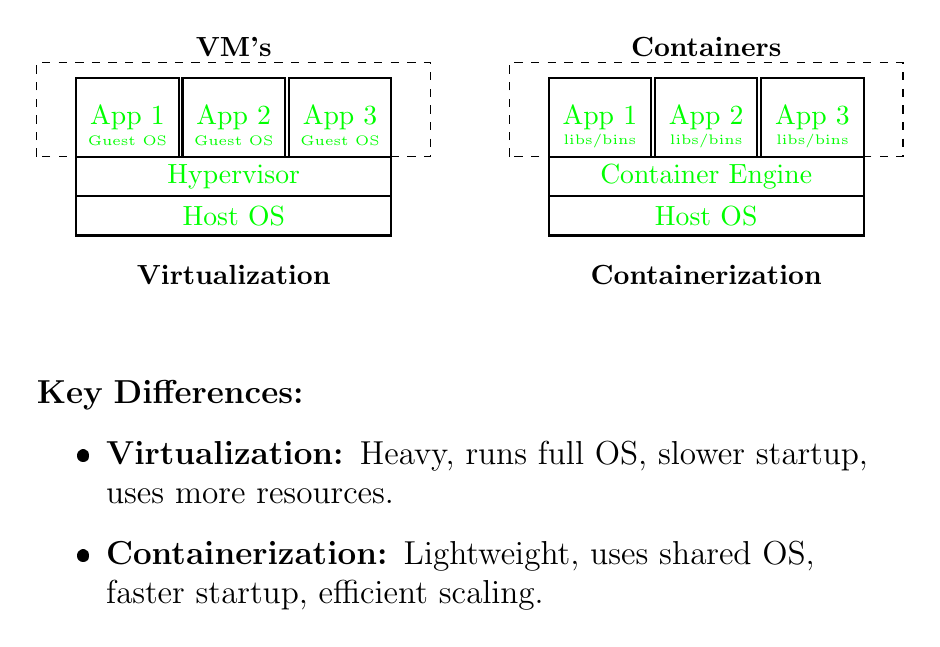
\begin{tikzpicture}

% Virtualization Diagram
% Host OS
\draw[thick] (0,0) rectangle (4,0.5);
\node at (2,0.25) {\textcolor{green}{Host OS}};

% Hypervisor
\draw[thick] (0,0.5) rectangle (4,1);
\node at (2,0.75) {\textcolor{green}{Hypervisor}};

% VM 1
\draw[thick] (0,1) rectangle (1.3,2);
\node at (0.65,1.5) {\textcolor{green}{App 1}};
\node at (0.65,1.2) {\textcolor{green}{\tiny Guest OS}};

% VM 2
\draw[thick] (1.35,1) rectangle (2.65,2);
\node at (2,1.5) {\textcolor{green}{App 2}};
\node at (2,1.2) {\textcolor{green}{\tiny Guest OS}};

% VM 3
\draw[thick] (2.7,1) rectangle (4,2);
\node at (3.35,1.5) {\textcolor{green}{App 3}};
\node at (3.35,1.2) {\textcolor{green}{\tiny Guest OS}};

% Label for VMs
\draw[dashed] (-0.5,1) rectangle (4.5,2.2);
\node at (2,2.4) {\textbf{\textcolor{black}{VM's}}};

% Virtualization Title
\node at (2,-0.5) {\textbf{\textcolor{black}{Virtualization}}};


% Containerization Diagram
% Host OS
\draw[thick] (6,0) rectangle (10,0.5);
\node at (8,0.25) {\textcolor{green}{Host OS}};

% Container Engine
\draw[thick] (6,0.5) rectangle (10,1);
\node at (8,0.75) {\textcolor{green}{Container Engine}};

% Container 1
\draw[thick] (6,1) rectangle (7.3,2);
\node at (6.65,1.5) {\textcolor{green}{App 1}};
\node at (6.65,1.2) {\textcolor{green}{\tiny libs/bins}};

% Container 2
\draw[thick] (7.35,1) rectangle (8.65,2);
\node at (8,1.5) {\textcolor{green}{App 2}};
\node at (8,1.2) {\textcolor{green}{\tiny libs/bins}};

% Container 3
\draw[thick] (8.7,1) rectangle (10,2);
\node at (9.35,1.5) {\textcolor{green}{App 3}};
\node at (9.35,1.2) {\textcolor{green}{\tiny libs/bins}};

% Label for Containers
\draw[dashed] (5.5,1) rectangle (10.5,2.2);
\node at (8,2.4) {\textbf{\textcolor{black}{Containers}}};

% Containerization Title
\node at (8,-0.5) {\textbf{\textcolor{black}{Containerization}}};

% Key Points Section
\node[align=left, text width=11cm, font=\large] at (5,-3.3) {
\textbf{Key Differences:}
\begin{itemize}
    \item \textbf{Virtualization:} Heavy, runs full OS, slower startup, uses more resources.
    \item \textbf{Containerization:} Lightweight, uses shared OS, faster startup, efficient scaling.
\end{itemize}
};

\end{tikzpicture}
\end{frame}

\section{Docker}
\begin{frame}
    \frametitle{\textbf{The Common Development Challenge}}

    \begin{columns}
        % Left Column: Description of the Problem
        \column{0.6\textwidth}
        \begin{itemize}
            \setlength\itemsep{1.5em}
            
            \item \textbf{\textcolor{red}{Project Complexity:}}  
            Developers use multiple technologies like React, Node.js, MongoDB, and more.

            \item \textbf{\textcolor{orange}{Evaluation Challenge:}}  
            Evaluators may not have all the required environments installed.

            \item \textbf{\textcolor{blue}{Key Question:}}  
            \textbf{How can the evaluator run the project without installing every dependency?}
        \end{itemize}

        % Right Column: Illustration of the Problem
        \column{0.4\textwidth}
        \begin{figure}
            \centering
            \includegraphics[width=0.9\linewidth]{Images/photo_2024-12-02_10-16-33.jpg}
            \caption{Different Technologies in a Project}
            \label{fig:dev-challenge}
        \end{figure}
    \end{columns}
    
    % Bottom Note
    \vspace{1em}
\end{frame}

\begin{frame}
    \frametitle{Solution}
    \centering
    \textbf{\textcolor{green!60!black}{Solution Insight:}}  
    \textit{Use Docker to containerize the project, ensuring portability and consistent environments!}
    \begin{figure}
        \centering
        \includegraphics[width=0.8\linewidth]{Images/docker_flowchart-1024x640.png}
        \caption{Caption}
        \label{fig:enter-label}
    \end{figure}
\end{frame}


\begin{frame}{Docker Introduction}
\begin{figure}
    \includegraphics[width=0.8\linewidth, height =0.5\linewidth ]{Images/platform-docker-logo.png}
    % \caption{Multiplicity of Goods and transportation}
    \label{fig:enter-label}
\end{figure}
\end{frame}


\begin{frame}
    \frametitle{\textbf{Docker}}
    
    \begin{columns}
        % Left Column: Shortened, Colorful Text
        \column{0.6\textwidth}
        \begin{itemize}
            \setlength\itemsep{1.5em}
            \item \textbf{\textcolor{orange}{Shipping container}} for code.
            \item \textbf{\textcolor{green}{Portable and self-sufficient}} app packaging.
            \item \textbf{\textcolor{purple}{Standardized operations}} enable automation.
        \end{itemize}
        
        % Right Column: Pictures
        \column{0.4\textwidth}
        \begin{figure}
            \centering
            \includegraphics[width=0.8\linewidth]{Images/dockercycle1.png}
            \caption{Docker container concept}
        \end{figure}
        
        \begin{figure}
            \centering
            \includegraphics[width=0.8\linewidth]{Images/dockerfile-2.png}
            \caption{Docker workflow}
        \end{figure}
    \end{columns}
    
\end{frame}




\begin{frame}{Basic Workflow}
\includegraphics[width=\textwidth,height=9cm]{Images/basic_workflow11 PM_2.png}
    
\end{frame}

\begin{frame}{Making Copies}

\includegraphics[width=\textwidth]{Images/basic_workflow3.png}

    
\end{frame}

\begin{frame}{Testing and Qualification}

\textbf{Before deploying a service update, it must undergo thorough testing and qualification to ensure reliability. To simplify testing and maintain confidence in quality, changes between updates should be minimal (operations objective).}
\begin{center}
\includegraphics[width=0.5\textwidth]{Images/ai_img1.png}
\end{center}

\end{frame}
\begin{frame}{Testing and Qualification}

\textit{However, this often conflicts with the need to patch and upgrade software to remain current (developer’s objective).}
\begin{center}
    

\includegraphics[width=0.6\textwidth]{Images/ai_img2.png}

\end{center}
\end{frame}

\begin{frame}{Update Example}

\textit{When updating a system, challenges often arise due to \textbf{dependency cascades}. A dependency cascade occurs when an update to one component (e.g., PostgreSQL) requires updates to other components (e.g., Memcached) or the server OS, which might not be immediately compatible.}

\begin{center}
    

\includegraphics[width=\0.7\textwidth]{Images/ai_img3.png}.

\end{center}
\end{frame}


\begin{frame}{Update Example}

    \begin{columns}
        % First column: Image
        \begin{column}{0.5\textwidth}
            \includegraphics[width=\textwidth]{Images/ai_imgTG1.jpg} % Replace 'example-image-a' with your image filename
        \end{column}

        % Second column: Text
        \begin{column}{0.5\textwidth}
            \textbf{Example:}
            \begin{itemize}
                \item Updating PostgreSQL might necessitate a newer version of Ubuntu, which in turn requires updating Memcached
                \item If the updated Memcached version is incompatible with existing middleware, it can trigger additional updates upstream, creating a cascading effect
                \item This highlights the importance of careful testing and qualification to balance stability and the need for advancements in software and systems.
            \end{itemize}
        \end{column}
    \end{columns}

% \textcolor{blue}{For example, updating PostgreSQL might necessitate a newer version of Ubuntu, which in turn requires updating Memcached. If the updated Memcached version is incompatible with existing middleware, it can trigger additional updates upstream, creating a cascading effect. This highlights the importance of careful testing and qualification to balance stability and the need for advancements in software and systems.
% }
    
\end{frame}



\begin{frame}{}
    \centering
    {\scalebox{10}{ \textcolor{red}{\textbf{?}}}} \\[1cm] % The large question mark
    {\Large \textit{What's the solution?}} % Text below the question mark
\end{frame}


\begin{frame}{Solution\#1}
    \begin{columns}
        % First column: Image
        \begin{column}{0.5\textwidth}
            \includegraphics[width=\textwidth]{Images/a-_imgTG2.jpg} % Replace 'example-image-a' with your image filename
        \end{column}

        % Second column: Text
        \begin{column}{0.5\textwidth}
            \textbf{Solution 1:}
            \begin{itemize}
                \item \textcolor{blue}{\textbf{Split Memcached and
PostgreSQL services onto different VMs.}}
                \item \textcolor{red}{\textbf{This would work but further complicates the deployment mesh and forces single-role-per VM policy, reducing flexibility}}
            \end{itemize}
        \end{column}
    \end{columns}
\end{frame}
% Solution #1: Split Memcached and
% PostgreSQL services onto different VMs.
% This would work but further complicates the deployment mesh and forces single-role-per VM policy, reducing flexibility
% • Solution #2: Containerise the PostgreSQL and Memcached services inside Docker




\begin{frame}{Solution\#2}
    \begin{columns}
        % First column: Image
        \begin{column}{0.5\textwidth}
            \includegraphics[width=\textwidth]{Images/ai_imgTG3.jpg} % Replace 'example-image-a' with your image filename
        \end{column}

        % Second column: Text
        \begin{column}{0.5\textwidth}
            \textbf{Solution 2:}
            \begin{itemize}
                \item {\Large \textit{\textbf{\textcolor{purple}{Containerize the PostgreSQL and Memcached services inside Docke}}}}
            \end{itemize}
        \end{column}
    \end{columns}
\end{frame}



\begin{frame}{How it Works}
    \begin{columns}
        % First column: Image
        

        % Second column: Text
        \begin{column}{0.5\textwidth}
            \textbf{Docker Basics:}
            \begin{itemize}
                \item \textcolor{blue}{\textbf{Developers use a base image, such as a specific version of Ubuntu, to build bespoke containers for hosting individual components like PostgreSQL.}}
                \item \textcolor{violet}{\textbf{These containers encapsulate all necessary elements, such as the OS version, libraries, updates, and application components.}}
            \end{itemize}
        \end{column}


        \begin{column}{0.5\textwidth}
            \includegraphics[width=\textwidth]{Images/ai_imgTG4.jpg} % Replace 'example-image-a' with your image filename
        \end{column}
    \end{columns}
\end{frame}


% Docker Basics:
% 	•	Developers use a base image, such as a specific version of Ubuntu, to build bespoke containers for hosting individual components like PostgreSQL.
% 	•	These containers encapsulate all necessary elements, such as the OS version, libraries, updates, and application components.





\begin{frame}{How it Works}
    \begin{columns}
        % First column: Image
        \begin{column}{0.5\textwidth}
            \includegraphics[width=\textwidth]{Images/ai_imgTG5.jpg} % Replace 'example-image-a' with your image filename
        \end{column}

        % Second column: Text
        \begin{column}{0.5\textwidth}
            \textbf{Container Functionality:}
            \begin{itemize}
                \item \textcolor{blue}{\textit{Docker transforms images into \textbf{running containers}, which are isolated OS instances within the host system.}}
                \item \textcolor{red}{\textit{Resources inside the container remain invisible to the external host system, ensuring operational isolation.}}

                \item \textit{Containers feature their own virtual networking layer, with automatically assigned IPs that are visible on the host system. TCP/IP port mapping and forwarding are supported for host-container communication.}
            \end{itemize}
        \end{column}
    \end{columns}
\end{frame}



	% •	Docker transforms images into running containers, which are isolated OS instances within the host system.
	% •	Resources inside the container remain invisible to the external host system, ensuring operational isolation.
	% •	Containers feature their own virtual networking layer, with automatically assigned IPs that are visible on the host system. TCP/IP port mapping and forwarding are supported for host-container communication.


\begin{frame}{Advanced Features}
    \begin{columns}
        % First column: Image
        

        % Second column: Text
        \begin{column}{0.5\textwidth}
            \textbf{Docker supports automated, script-driven image generation through a Dockerfile, which specifies:}
            \begin{itemize}
                \item \textcolor{blue}{\textbf{The base Linux image.}}
                \item \textcolor{orange}{\textbf{Software installation commands.}}
                \item \textcolor{violet}{\textbf{Exposed TCP/IP ports.}}
                \item \textcolor{red}{\textbf{Default commands to execute upon container launch.}}
            \end{itemize}
        \end{column}


        \begin{column}{0.5\textwidth}
            \includegraphics[width=\textwidth]{Images/ai_imgTG6.jpg} % Replace 'example-image-a' with your image filename
        \end{column}
    \end{columns}
\end{frame}




%Arpita
% \Section{The Good, the Bad and the Interesting of Docker}
\begin{frame} % Use "plain" to remove headers/footers
    \centering
    {\Huge \textbf{\underline{The Good, the Bad and}} \\[10pt]
     \textbf{\underline{the Interesting of}} \\[10pt]
     \textbf{\underline{Docker}}}
\end{frame}

% Slide 2: THE GOOD (Black Background)
\begin{frame} % Use "plain" to remove headers/footers
    \centering
    {\Huge \textbf{\underline{THE GOOD}}}
\end{frame}
% First "Good part of Docker" slide




\begin{frame}
 {\Huge \textbf{Good part of Docker}}\\[15pt]
    \begin{columns}
        % First Column: Text Description
        \column{0.5\textwidth}
        \centering
        \color{black}
       
        \color{black}
        \begin{itemize}
            \item {\underline{Portability:}}\\[2pt]
            \begin{itemize}
                \item<1-1>Docker containers encapsulate an application and its dependencies.\\[5pt]
                \item<2->making it easy to move the app across different environments.
            \end{itemize}
           
        \end{itemize}

        % Second Column: Illustration
        \column{0.5\textwidth}
        \centering
        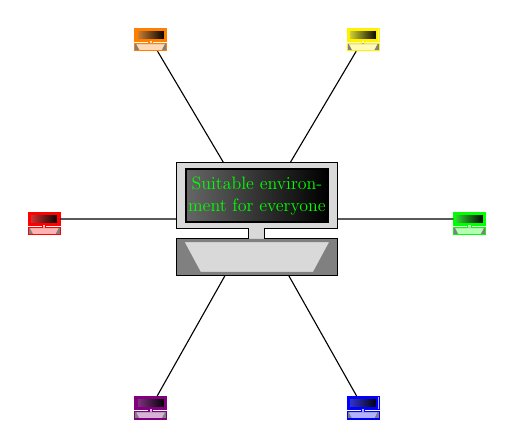
\begin{tikzpicture}[scale=0.45, every node/.style={transform shape}]
            % Central Docker Application
            \pic(comp0) [
                draw,
                fill = gray!30,
                pic text = {Suitable environment for everyone}
            ] {computer};

            % Different Environments
            \path(comp0-c.center) pic 
                foreach[count=\i] \farbe/\label in {
                    yellow/Development,
                    orange/Testing,
                    red/Staging,
                    red!50!blue/Production,
                    blue/Cloud (AWS),
                    green/On-Premises
                }
                (comp\i) [
                    draw = \farbe,
                    fill = \farbe!30,
                    display/.append style = {left color=\farbe!80!black!80},
                    scale = 0.2,
                ] at +(60*\i:6) {computer};

            % Connect Environments to Docker Application
            \foreach \i in {1,2,4,5} \draw (comp\i-c) -- (comp0-c);
            \foreach \i in {3,6} \draw (comp\i-m) -- (comp0-c);
        \end{tikzpicture}
    \end{columns}
\end{frame}



% Second "Good part of Docker" slide with image
\begin{frame}
    \centering
    \color{black}
    {\Huge \textbf{Good part of Docker}}\\[15pt]
    \color{black}
    \begin{columns}
        \begin{column}{0.5\textwidth}
            \begin{itemize}
                \item {\underline{Isolation:}}\\[2pt]
                \begin{itemize}
                    \item<1-1> Docker provides a high level of isolation. \\[5pt]
                    \item<2-> Containers can run independently without affecting other processes.
                \end{itemize}
              
            \end{itemize}
        \end{column}
        \begin{column}{0.35\textwidth}
            \centering
            \includegraphics[width=\textwidth]{isolation.png} % Replace with your image path
        \end{column}
    \end{columns}
\end{frame}

% Third "Good part of Docker" slide with TikZ diagram
\begin{frame}
    \centering
    \color{black}
    {\Huge \textbf{Good part of Docker}}\\[15pt]
    \color{black}
    \begin{columns}
        \begin{column}{0.5\textwidth}
            \begin{itemize}
                \item {\underline{Simplifies CI/CD:}}\\[2pt]
                Docker is a key enabler for Continuous Integration and Continuous Deployment (CI/CD).  \\[5pt]
            \end{itemize}
        \end{column}
        \begin{column}{0.6\textwidth}
            \centering
            \begin{tikzpicture}
                \arrows[0.8];  % TikZ diagram for CI/CD fitting
            \end{tikzpicture}
        \end{column}
    \end{columns}
\end{frame}

\begin{frame}{Docker Benefits in a nutshell}
    \centering
    \resizebox{0.7\textwidth}{!}{ % Resize the diagram to 70% of the text width
        \smartdiagram[constellation diagram]{
            Good side of Docker,
            Portability, Isolation, Efficient Resource Usage, Simplifies CI/CD, Scalability
        }
    }
\end{frame}



\begin{frame} % Use "plain" to remove headers/footers
    \centering
    {\Huge \textbf{\underline{THE INTERESTING}}}
\end{frame}

\begin{frame}
    \centering
    \color{black}
    {\Huge \textbf{Interesting part of Docker}}\\[15pt]
    \color{black}
    \begin{columns}
        \begin{column}{0.5\textwidth}
            \begin{itemize}
                \item {\underline{Microservices Architecture:}}\\[2pt]
                \begin{itemize}
                    \item<1-1>   Containers allow each microservice to be packaged, tested, and deployed independently  \\[5pt]
                    \item<2->speeds up development and deployment cycles.
                \end{itemize}
               
            \end{itemize}
        \end{column}
        \begin{column}{0.5\textwidth}
            \centering
            \includegraphics[width=\textwidth]{VMC-Microservices-3.png} % Replace with your image path
        \end{column}
    \end{columns}
\end{frame}
\begin{frame}
    \centering
    \color{black}
    {\Huge \textbf{Interesting part of Docker}}\\[15pt]
    \color{black}
    \begin{columns}
        \begin{column}{0.5\textwidth}
            \begin{itemize}
                \item {\underline{Integration with Cloud Providers:}}\\[2pt]
                Docker integrates well with cloud providers like AWS, Google Cloud, and Azure. \\[5pt]
            \end{itemize}
        \end{column}
        \begin{column}{0.5\textwidth}
            \centering
            \begin{tikzpicture}[scale=0.3]  % Scale down the whole diagram to 40% of original size
                % Cloud Services (Compute, Storage, Backup)
                \node[service, fill=computeorange] (compute) at (-4,-2) {Compute Service};
                \node[service, fill=storageyellow] (storage) at (4,-2) {Storage Service};
                \node[service, fill=backupgray] (backup) at (0,-3.5) {Backup Service};

                % Clients
                \node[client] (client1) at (-6,3) {Client 1};
                \node[client] (client2) at (0,3) {Client 2};
                \node[client] (client3) at (6,3) {Client 3};

                % Security Components (Firewall & VPN)
                \node[firewall] (firewall) at (0,-5.5) {Firewall / VPN};

                % Connections between clients and cloud infrastructure
                \path[connection] (client1) edge (cloud);
                \path[connection] (client2) edge (cloud);
                \path[connection] (client3) edge (cloud);

                % Connections between cloud infrastructure and cloud services
                \path[connection] (cloud) edge (compute);
                \path[connection] (cloud) edge (storage);
                \path[connection] (cloud) edge (backup);

                % Data connections between services
                \path[dataconnection] (compute) edge (storage);
                \path[dataconnection] (compute) edge (backup);
                \path[dataconnection] (storage) edge (backup);

                % Connections from cloud to security component
                \path[connection] (cloud) edge (firewall);
                \path[connection] (compute) edge (firewall);
                \path[connection] (storage) edge (firewall);
                \path[connection] (backup) edge (firewall);

                % Security connections from clients to firewall
                \path[dataconnection] (client1) edge (firewall);
                \path[dataconnection] (client2) edge (firewall);
                \path[dataconnection] (client3) edge (firewall);
            \end{tikzpicture}
        \end{column}
    \end{columns}
\end{frame}
\begin{frame}
    \centering
    \color{black}
    {\Huge \textbf{Interesting part of Docker}}\\[15pt]
    \color{black}
    %\begin{columns}
        %\begin{column}{0.5\textwidth}
            \begin{itemize}
                \item {\underline{Docker Hub:}}\\[2pt]
                \begin{itemize}
                    \item<1-1>  Docker Hub is a public repository\\[5pt]
                    \item<2->It's a great resource for finding pre-built containers for common services.
                \end{itemize}
                
            \end{itemize}
       % \end{column}
        %\begin{column}{0.8\textwidth}
            \centering
            \includegraphics[width=0.5\textwidth]{dock-8-11-min.JPG} % Replace with your image path
        %\end{column}
    %\end{columns}

    
\end{frame}

\begin{frame} % Use "plain" to remove headers/footers
    \centering
    {\Huge \textbf{\underline{THE BAD}}}
\end{frame}


\begin{frame}
    \centering
    \color{black}
    {\Huge \textbf{Bad part of Docker}}\\[15pt]
    \color{black}
   
            
       \begin{itemize}
                \item<1-1> {\underline{Overhead in Small Projects:}}\\[2pt]
              For small applications or simple setups, Docker might add unnecessary overhead.\\[5pt]

            
            \end{itemize}
            \end{frame}
\begin{frame}
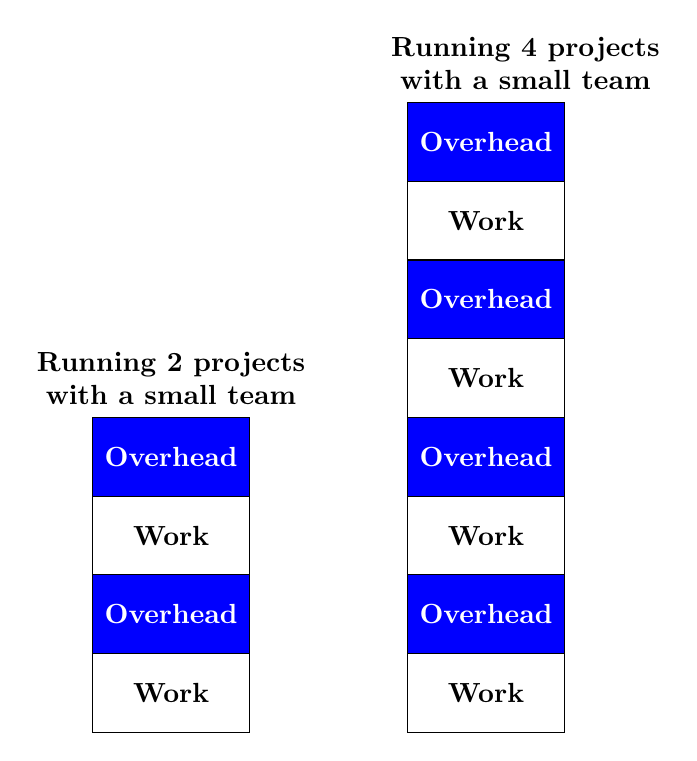
\begin{tikzpicture}
% First frame: Running 2 projects
\node at (1, 4.5) [align=center] {\textbf{Running 2 projects}\\ \textbf{with a small team}};
\draw (0, 0) rectangle ++(2, 1) node[midway] {\textbf{Work}};
\draw[fill=blue, text=white] (0, 1) rectangle ++(2, 1) node[midway] {\textbf{Overhead}};
\draw (0, 2) rectangle ++(2, 1) node[midway] {\textbf{Work}};
\draw[fill=blue, text=white] (0, 3) rectangle ++(2, 1) node[midway] {\textbf{Overhead}};

% Second frame: Running 4 projects
\node at (5.5, 8.5) [align=center] {\textbf{Running 4 projects}\\ \textbf{with a small team}};
\foreach \y in {0, 2, 4, 6} {
    \draw (4, \y) rectangle ++(2, 1) node[midway] {\textbf{Work}};
    \draw[fill=blue, text=white] (4, \y+1) rectangle ++(2, 1) node[midway] {\textbf{Overhead}};
}
\end{tikzpicture}
\end{frame}

\begin{frame}
    \centering
    {\Huge \textbf{Bad part of Docker}}\\[15pt]
    \color{black}

  \begin{itemize}
                \item {\underline{Network Complexity:}}\\[2pt]
               Docker's networking system can be difficult to configure and troubleshoot, especially when containers need to communicate with each other across different hosts or external services.\\[5pt]
            \end{itemize}

            \end{frame}






% Advanced Features:
% 	•	Docker supports automated, script-driven image generation through a Dockerfile, which specifies:
% 	•	The base Linux image.
% 	•	Software installation commands.
% 	•	Exposed TCP/IP ports.
% 	•	Default commands to execute upon container launch.

\end{document}
